\section{Current Accomplishment}
The system currently can listen to audio command via a simple GUI interface built on PyQt. This content will be sent to the Google Cloud service to get back the text form. System currently supports 2 intents: forward/backward movement and left/right turn. These actions along with its parameters (angle to turn, distance to move) are analyzed and mapped to program that controls the robot. There is another GUI simulator that draws the movement at the same time. Current setup is illustrated in figure \ref{fig:currentSetup}.
\begin{figure}[tb]
\centering
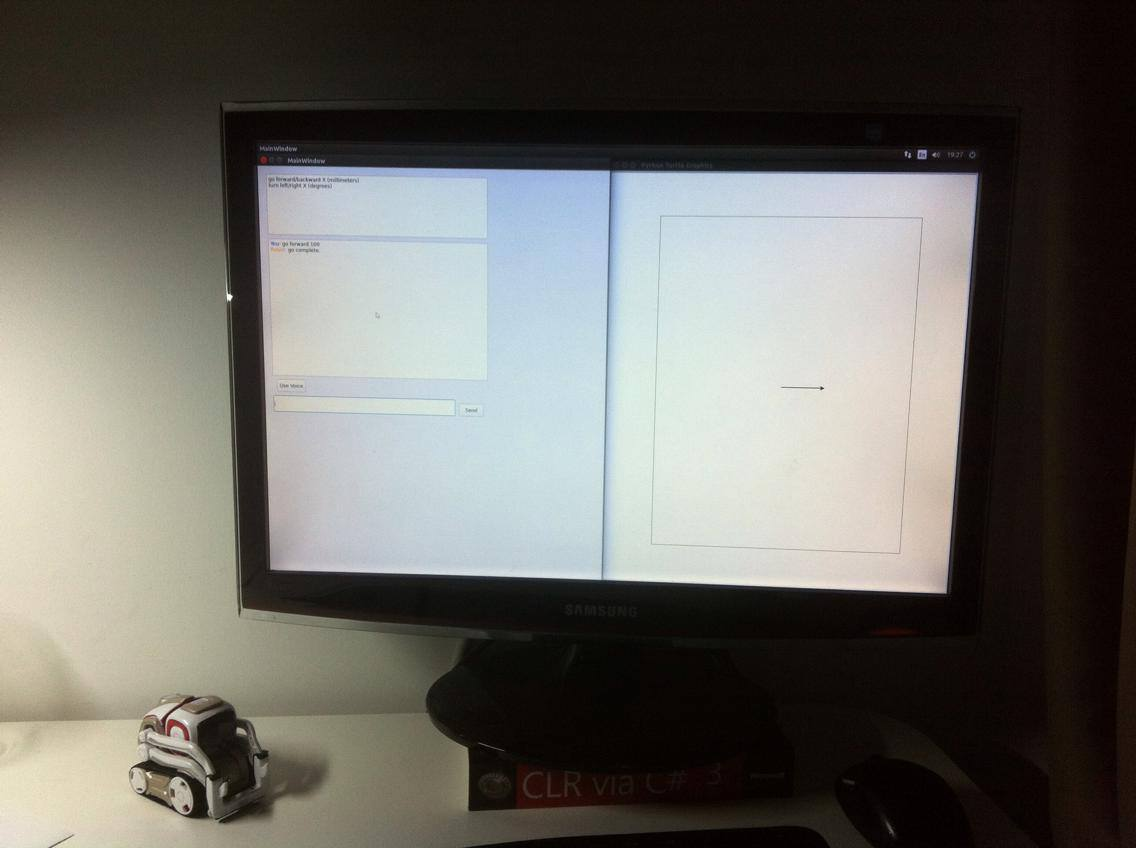
\includegraphics[width = 1.0\hsize]{./figures/currentSetup}
\caption{Current setup of the project: a Cozmo robot (on the left) is connected wirelessly through a mobile device. The program has a simple GUI that can take input in both audio and text formats. Command is analyzed and sent to both robot and a drawing simulator (on the right).}
\label{fig:currentSetup}
\end{figure}

Below is the list of activities to achieve this current state:
\begin{enumerate}
	\item Main Interface:
	\begin{itemize}
		\item Use Python and PyQt to build a simple GUI where the commands can be recorded or typed. It's similar to a chat application between human and robot.
		\item Integrate the GUI with other components of the system: simulator, robot, speech recognition etc.		
	\end{itemize}
	\item Automatic Speech Recognition system:
	\begin{itemize}
		\item Test ASR systems to choose the best one: CMUSphinx, Kaldi, Nervana DeepSpeech, Google Cloud Speech service (the winner)
		\item Signup and Setup Google Cloud client API.
		\item Write code to capture audio input then communicate with Google Cloud service (send request then analyze feedback).		
	\end{itemize}
	\item Information Extractor:
	\begin{itemize}
		\item Attempt to use Part-Of-Speech tags to extract information. However this did not work appropriately in this specific context where commands are spoken, not natural language. 
		\item Apply a set of synonyms to the text input. This eases the processing step: input with specific words corresponds to a unique intent.
		\item Currently, the goal is to build command-oriented system, hence string processing fits well to extract the intent and related parameters.
	\end{itemize}
	\item Robot:
	\begin{itemize}
		\item Search for a robot that can not only fulfill our demands (movement) but also provide other functionalities (built-in camera, built-in speaker, etc.).
		\item In the mean time, build a drawing simulator to test ASR and IE systems.
		\item Get Cozmo robot that fits well with the requirement: it has motors, camera, speaker, LED display, etc. and it's programmable via the SDK \cite{ANKI:2017}.
		\item Install SDK and some other libraries to connect Linux post to the mobile device which controls Cozmo wirelessly.
	\end{itemize}
\end{enumerate}

\section{Problems and Solutions}
\subsection{ASR system}
Firstly, I wanted a open-source and offline solution for the automatic speech recognition system. I tried out several solutions and also thinked of implementing my own ASR system with deep learning. However, there were a few problems for this approach:
\begin{enumerate}
	\item As a non-native speaker, I found open-source software for ASR like CMUSphinx \cite{CMUSphinx:2017} and Kaldi \cite{Kaldi:2017} are not good enough. For example, I often get "tune rite" when I say "turn right". In addition, it's not easy to use these libraries. We have to go through long process of installation and we hardly find documentations about their usage.
	\item To build an ASR system from scratch using deep learning is feasible but we would be unlikely to have a good ASR system at the level of Amazon Alexa, Apple Siri or Google Speech. The main reason is the lack of data and powerful ressource for training.
\end{enumerate}
Therefore, I decided to use Google Cloud speech service \cite{GoogleCloud:2017}. It is robust and easy to use: using its API, we send the audio content to the service and get back the text. One trade-off is the internet connection requirement and the system must be authorized to use Google Cloud service. However, it cuts the computation cost of using an ASR server locally. Note that state of the art ASR system uses deep neural network which requires massive computations.

\subsection{Information Extraction}
Initially, I started processing the text input with the traditional approach where natural language processing tools are used. Given a sentence, I used Part-Of-Speech (POS) tagger to tag each word into categories like verb, nouns, number, adverb, adjective, etc. And based on these tags, I could determine the action (the verb), and its parameters (number, nouns). However, there were a few problems as follow:
\begin{enumerate}
	\item There is no perfect POS tagger and its performance depends on its training data. Hence, it did not show good result in tagging command sentences (which hardly appear in training corpus).
	\item For movement, people tend to use short commands such as: "backward X metres", "turn left" (the angle is 90 degree implicitly). Unfortunately, many of these short commands do not form a complete sentence and POS tagger can not perform well on incomplete sentences.
	\item The behavior of POS taggers are unpredicted and inconsistent. A minor change in input can lead to total different (and wrong) tags. This does not fit well with voice system where people can make minor grammatical mistakes or paralanguage ("um", "uh" utterances).
\end{enumerate}
Therefore, I switched to use a simpler string processing: 
\begin{enumerate}
	\item First of all, text input will be preprocessed by removing meaningless words like: please, can you, etc.
	\item Secondly, a synonyms set will be applied to replace similar words to its specific key word. 
	\item Finally, a search with some predefined rules is performed to extract the intent and its parameters.
\end{enumerate}
This seems to be more robust (no POStagging) than the first approach. And it fits well with the general goal of this application: say short order and robot acts correspondingly.

\subsection{Main Interface}
The system needs to host interaction between human and robot. Therefore a graphical user interface (GUI) must to be built. It brings numerous advantages: storing the dialogue history, enabling voice-command whenever the user wants by just clicking a button, etc. There are several difficulties:
\begin{enumerate}
	\item Coding up Python GUI application involves using tools as TkInter or PyQt. And learning how to use these libraries takes time.
	\item The system is composed of multiple blocks. In order to have a smooth interface, I need to use threading in some tasks, for example: one thread records voice command, another thread communicates with Google Cloud service, etc. 
\end{enumerate}
All these are technical difficulties and I solved them through many trials and errors.